\chapter{Introducción}

En este primer punto, describiremos la importancia del correcto diagnóstico del cáncer de piel, y de sus dificultades de detección. Analizaremos la justificación del motivo de realización de este TFG, así como los objetivos a cumplir y la planificación seguida en su desarrollo.

\section{Motivación}

El cáncer es una de las causas de muerte principales en el mundo. Su gran agresividad, así como su dificultad de diagnóstico, debido a su gran variedad de ubicaciones y manifestaciones, provoca que un alto porcentaje de casos no sean diagnosticados a tiempo correctamente. Tan solo en 2023, aproximadamente se registraron 20 millones de nuevos casos de cáncer a nivel mundial, y produciéndose algo menos de 10 millones de defunciones \cite{cancerincidence}.\\

Estos registros provocan una gran inquietud en la población y entre los expertos de la materia; debido al aumento que se produce cada año, se espera que para el año 2050, el número de nuevos casos sea un 77\% mayor \cite{cancerprevision}.  Por desgracia, no existen formas de prevención claras para este tipo de enfermedad, ni un tratamiento efectivo que permita al paciente recuperarse fácilmente. \\

La única opción probada es la realización de pruebas rutinarias a colectivos de riesgo, para así acelerar la detección de posibles tumores, y aumentar la esperanza de supervivencia. Esto se ve reflejado en las cifras de los dos tipos de cáncer más frecuentes: el cáncer de mama, y el cáncer colorrectal. Si se detectan en fases iniciales, la correcta recuperación del colon podría aumentarse hasta el 90\% \cite{coloncancer}, mientras que en el cáncer de mama, podría reducirse su mortalidad entre un 25-31\%. Gracias a la existencia de pruebas rutinarias programadas por servicio de salud, se puede reducir la mortalidad.\\

El gran problema de estos tipos de cánceres son la escasa visibilidad y síntomas de los mismos; cuando muestran señales, es probable que la tasa de supervivencia sea mucho menor, sobre todo en el colon. Pero existe otro tipo de cáncer que sí se manifiesta de forma más visible y que puede alarmar al paciente de forma más temprana: el cáncer de piel.\\

Este tipo de tumores puede manifestarse en las diferentes capas de la dermis, y su origen se atribuye a la exposición prolongada a la luz solar sin hacer uso de protección. Debido a los daños que sufre la capa de ozono, y otros factores ambientales, la cantidad de rayos ultravioleta que llegan hasta la superficie ascendió desde que se tienen registros. Si bien la capa de ozono parece recuperarse, debemos ser cautos, y tener cuidado de nuestra piel; los rayos ultravioleta pueden dañar células de la misma, y provocar alteraciones en su material genético. Su principal consecuencia es el crecimiento incontrolado de células, origen de los tumores cancerígenos en la piel.\\

Se estima que en el mundo, los tumores de la piel representan un tercio de los casos de cáncer diagnosticados. Esta distribución sigue valores parecidos en España, y al igual que las cifras de otros tipos de tumores, los casos diagnosticados aumentan año tras año. Las muertes debidas a esta enfermedad son principalmente, por ser identificadas en fases tardías de su evolución. Debido a que la piel es el órgano más grande del cuerpo humano, y que está en contacto con todos los capilares sanguíneos y el sistema linfático, las células cancerosas se pueden extender por ellos hacia otros lugares del cuerpo.\\

Aunque este cáncer puede ser identificado de forma más sencilla por su portador, la escasa información acerca del tema, y la confusión con otras lesiones benignas de la piel como verrugas o lunares, provoca una disminución en las posibilidades de supervivencia. Por ello, el objetivo de este trabajo es aportar una nueva forma de diagnóstico que permita a los usuarios obtener una orientación acerca de qué posible lesión están experimentando en la piel, y sirva como complemento del experto. O bien, ayudar a los expertos a tomar la decisión, acortando los tiempos de diagnóstico para aumentar las posibilidades de supervivencia. Esta tarea será realizada gracias al uso de una de las herramientas en auge en la actualidad: la inteligencia artificial, y concretamente, el uso de deep learning y métodos de visión por computador.\\
 
 Mediante una nueva arquitectura, el propósito es conseguir un modelo capaz de segmentar las manchas de interés en la piel que estén recogidas en una fotografía. Dicha fotografía será capturada con el teléfono móvil del usuario, retirando así la necesidad de disponer de dispositivos especializados. Y posteriormente, clasificar dichas manchas para ofrecer al usuario final una respuesta sólida acerca del posible tipo de lesión de piel que sufre.\\

\newpage
\subsection{El cáncer de piel}

Prosiguiendo con el estudio inicial, el diagnóstico del cáncer de piel  \cite{cancerpieltipos}, se dificulta, sobre todo, por su amplia variedad de formas, tamaños, texturas y manifestaciones. Aunque su visibilidad pueda parecer evidente, (ya que es observable a nivel macroscópico) puede ser confundido fácilmente con lesiones benignas. Normalmente, suele dividirse entre dos tipos diferentes:
\begin{itemize}
	\item \textbf{Melanomas de la piel}. Son la variante más peligrosa. Su origen se encuentra en los melanocitos, las células encargadas de dar el color bronceado a la piel.  Estas pueden comenzar a crecer sin control originando tumores, los cuales crecen y se diseminan rápidamente hacia otras regiones del organismo, provocando la metástasis, una extensión a nivel total del organismo. Es el más grave de los diagnósticos. Puede identificarse como una mancha oscura en la piel, formando tumores de color café oscuro. Sin embargo, debido a la gran variedad de reacciones, pueden darse de color rosado si dejan de producir melanina. Este aspecto dificulta su diagnóstico, por lo que el papel de las herramientas de visión por computador pueden ayudar a su identificación.
	\item \textbf{Cánceres no melanomas}. Este tipo de cánceres no se ubican en los melanocitos, y pueden ser tratados mediante otras ténicas menos agresivas debido a su rara probabilidad de expansión. Los más comunes, son los tumores de células basales y los de células escamosas:
	\begin{itemize}
		\item \textit{Células basales}. Componen la capa inferior de la piel, y son las células encargadas de sustituir aquellas que componen la capa más externa de la piel. Se encuentran , por tanto, en constante reproducción para cubrir aquellas que mueren en la superificie. Si experimentan alguna mutación, producen tumores de color similar a la piel del paciente, con la posibilidad de aparecer en colores como negro brillante en las pieles más oscuras.
		
		\item \textit{Células escamosas}. Son las células externas de la piel, con forma plana. Se regeneran constantemente gracias a las células basales, que producen estas células las cuales se aplanan a medida que ascienden hacia la capa externa. Es frecuente, de nuevo, en zonas expuestas al sol, sobre todo la cara. Normalmente, se encuentran bien localizados, y puede procederse a su extirpación. En casos en los que se haya extendido, se hace uso de radioterapia.
		
	\end{itemize}
\end{itemize}

Aunque en base a su descripción parezcan distinguibles, son fácilmente confundidos por su variedad con otros tumores benignos de la piel, como:

\begin{itemize}
	\item \textbf{Lunares}. Conocidos médicamente con nevus, se trata de hiperpigmentación benigna en la piel.
	\item \textbf{Verrugas}. Tumores benignos de piel, frecuente debido a virus como el del papiloma humano.
	\item \textbf{Lesiones vasculares}. Varices, derrames, y otro tipo de problemas circulatorios.
	\item \textbf{Lipomas}. Tumores de tacto blando, debido a su contenido en lípidos (grasa).
	\item \textbf{Queratosis seborreica}. Son manchas cerosas, comúnmente desarrolladas en la espalda. De aspecto oscuro y gran relieve, no suponen ninguna amenaza más allá de posible incomodidad al roce o estética.
\end{itemize}

El uso de deep learning para este fin resulta interesante como forma de mejora del diagnóstico ante casos malignos y benignos de gran similitud, los cuales pueden confundir y dificultar la labor incluso a expertos dermatólogos.

\subsection{Dificultades del diagnóstico}

Existe una gran dificultad de conocer la naturaleza del tumor del paciente. Habitualmente, se suele extraer una muestra del tejido afectado para proceder a su análisis en laboratorio. A esta técnica se le denomina biopsia.\\

Es un proceso efectivo, que consiste en el estudio bajo microscopio de las células extraídas, y el patrón que constituye el tejido. Su proceso más complejo es la extracción, ya que si ésta no se realiza correctamente, ciertas células cancerígenas pueden no aparecer en la muestra y realizarse un diagnóstico erróneo. Además, debido a la falta de especialistas en la materia que puedan realizar las incisiones, personal médico no cualificado en esta materia suele realizar su extracción. Se estipula que en lesiones inflamatorias, el correcto estudio de la patología se da en el 77\% de los casos si la muestra es recogida por un dermatólogo, y un 41\% si la realiza un ayudante \cite{LLAMASVELASCO201212}.\\

Existen varias técnicas: mediante corte con tijera, mediante rasurado, extracción mediante bisturí, o en forma elíptica, persiguiendo la extracción total de la lesión. En el caso de las dos primeras opciones, solo está indicada si la lesión es superficial y no existe riesgo de que se trata de un melanoma por las complicaciones que esto conlleva de una posible diseminación y metástasis. \\

Aunque esta técnica suele ofrecer buenos resultados, debido a que la distinción entre un tumor de tipo melanoma y un simple nevus puede ser complicada, sería de interés conocer una evaluación previa. Y es aquí donde podemos ver la utilidad del proyecto propuesto: se busca reforzar el diagnóstico del experto utilizándose un modelo de aprendizaje.\\

También hay que tener en cuenta otros factores que pueden perturbar el diagnóstico tradicional, como lo es la correcta manipulación de la muestra extraída, y su coloración adecuada para mejorar el contraste del tejido y poder distinguir el patrón descrito por las células y su núcleo. Además, la herida dejada en la piel puede sufrir complicaciones como hemorragias o infecciones si no se tratan adecuadamente. Reducir por tanto este tipo de operaciones a las estrictamente necesarias gracias a un modelo de aprendizaje profundo es una opción atractiva.

\section{Justificación}

Debido a la necesidad de facilitar el acceso al diagnóstico de forma orientativa, sin necesidad  de medios tecnológicos especializados, surge la necesidad de algún medio de diagnóstico gratuito capaz de acelerar el proceso mediante la prognosis, y reducir la tasa de mortalidad de la enfermedad. Encontramos, de esta forma, un área de conocimiento poco explorada: la creación de una aplicación móvil, capaz de emplear modelos detección y prognosis de cáncer de piel, empleando mecanismos específicos para dispositivos de baja potencia.

Los smartphones, al tratarse de un dispositivo altamente extendidos en la sociedad, pueden servir como un medio clave a la hora de extender modelos de salud críticos como el de diagnóstico de enfermedades cancerosas. De esta forma, podríamos acortar los largos tiempos de espera, realizando un diagnóstico previo para declarar cuáles son los casos que requieren mayor prioridad médica.

Sin embargo, no existen modelos de este ámbito lo suficientemente ligeros como para ser portados de forma local dentro del propio terminal, que no necesiten de conexión a Internet, y que velen por la seguridad y privacidad de los datos. Esto convierte el problema en una interesante temática de investigación, la cual será tratada en este documento.

\section{Objetivos}
\label{cap:objetivos}

Teniendo en cuenta los factores estudiados acerca de la enfermedad en los puntos anteriores, y las carencias del estado del arte actual, podemos afirmar que el uso de un modelo de aprendizaje profundo en dispositivos de potencia reducida permite:
\begin{enumerate}
	\item Facilitar la toma de decisiones de los expertos dermatólogos en casos complicados, a modo de sistema de ayuda a la toma de decisiones.
	\item Defender la utilidad de los modelos de aprendizaje profundo en el estudio y evaluación de casos en el ámbito médico, siendo en este caso la identificación de la patología a nivel macroscópico, sin necesidad de realizar una biopsia con el posible riesgo que esto conlleva.
	\item Crear una base de datos robusta y completa capaz de representar adecuadamente la población real de la enfermedad, partiendo, para ello, de la construcción de un conjunto de datos mediante una técnica no explotada en el estado del arte: la fusión de conjuntos de imágenes.
	\item Realizar, mediante un enfoque novedoso, el entrenamiento de un modelo con dos niveles de modelos especializados: uso de clasificación binaria para prediagnóstico de la enfermedad, y especificación de la misma mediante modelos especializados separados para enfermedades benignas y malignas, empleando la cuantización como método de simplificación.
	\item Mejorar la accesibilidad, al hacer uso de un dispositivo esencial en nuestra vida diaria como por ejemplo, los teléfonos móviles, aprovechando la posibilidad de que la manifestación de los tumores de piel son visibles a nivel macroscópico.
	\item Mostrar el desempeño de los modelos cuantizados y simplificados mediante el uso de una aplicación para dispositivos Android, capaz de ejecutarlos y mostrar su funcionamiento.
\end{enumerate}

En este documento, estudiaremos el estado del arte actual, y analizaremos e implementaremos una aplicación para dispositivos móviles que sea capaz de realizar la segmentación de la mancha cutánea, y su posterior clasificación dentro de una lista de patologías posibles. Se busca informar al usuario del riesgo de su lesión, y de su posible diagnóstico final, el cual debe ser verificado por el experto. De esta forma, el software final puede contribuir a acelerar los diagnósticos de esta enfermedad,  y favorecer la esperanza de vida de los pacientes en caso de que su lesión sea cancerosa.

Adicionalmente, se incluyen dos repositorios en los que se incluye información acerca de los datos empleados y los modelos entrenados\footnote{Datos: \url{https://github.com/hexecoded/TFG}}, y la aplicación realizada\footnote{Aplicación: \url{https://github.com/hexecoded/TFG-Android}}, de forma que se pueda contribuir en su desarrollo y realizar nuevas mejoras en trabajos futuros.

\section{Planificación}

La planificación de este proyecto se ha realizado teniendo en cuenta la necesidad de alcanzar pequeños objetivos de forma frecuente, para avanzar de forma firme y segura descartando la mínima cantidad de trabajo realizado. Esto coincide de forma directa con la filosofía de trabajo Scrum~\cite{schwaber2011scrum}, que tiene en cuenta los siguientes elementos:

\begin{enumerate}
	\item Puesta en valor de avances ejecutables y mostrables, mediante pruebas correctamente realizadas.
	\item Entregas periódicas, donde se ofrezca de forma visual y tangible los avances realizados.
	\item Reuniones cada cortos periodos de tiempo, para evaluar los progresos alcanzados y proponer las siguientes tareas a realizar.
\end{enumerate}

Si bien se ha priorizado la aplicación de este mecanismo de trabajo, también se ha combinado con el establecimiento en períodos concretos dedicados a ciertas áreas de trabajo, como el estudio del estado del arte, el preprocesado de datos, los modelos, la cuantización o el desarrollo en Android, sin olvidar la documentación del proyecto en la memoria. Esto se debe a que fases como el entrenamiento de modelos no se entenderían sin el estudio del estado del arte o el preprocesado de datos.

De esta forma, podemos resumir el tiempo dedicado a cada una de las tareas en la tabla \ref{tab:planif}, donde se describen los intervalos de tiempo dedicados a cada sección del proyecto.

\begin{table}[H]
	\centering
	\begin{tabular}{|c|c|c|}
		\hline
		\textbf{Fase} & \textbf{Inicio} & \textbf{Fin} \\ \hline
		Valoración de temáticas a elegir para el TFG & 15/09/23 & 03/10/23 \\ \hline
		Estudio y valoración del estado del arte & 03/02/24 & 24/04/24 \\ \hline
		Preprocesado de datos & 07/02/24 & 18/04/24 \\ \hline
		Entrenamiento de modelos & 14/02/24 & 31/05/24 \\ \hline
		Cuantización & 31/05/24 & 14/06/24 \\ \hline
		Desarrollo de la aplicación & 20/05/24 & 20/06/24 \\ \hline
		Escritura de la memoria & 08/06/24 & 22/06/24 \\ \hline
	\end{tabular}
	\caption{Tabla de tiempos de trabajo}
	\label{tab:planif}
\end{table}

Teniendo en cuenta únicamente los aspectos relacionados con el desarrollo de este TFG, este se ha llevado a cabo dando lugar al diagrama de Gantt de la figura \ref{fig:gantt}, donde la semana uno (S1) se corresponde a la semana del 3 de febrero, y la última, S19, a la semana del 17 de junio.

\begin{figure}[H]
	\centering
	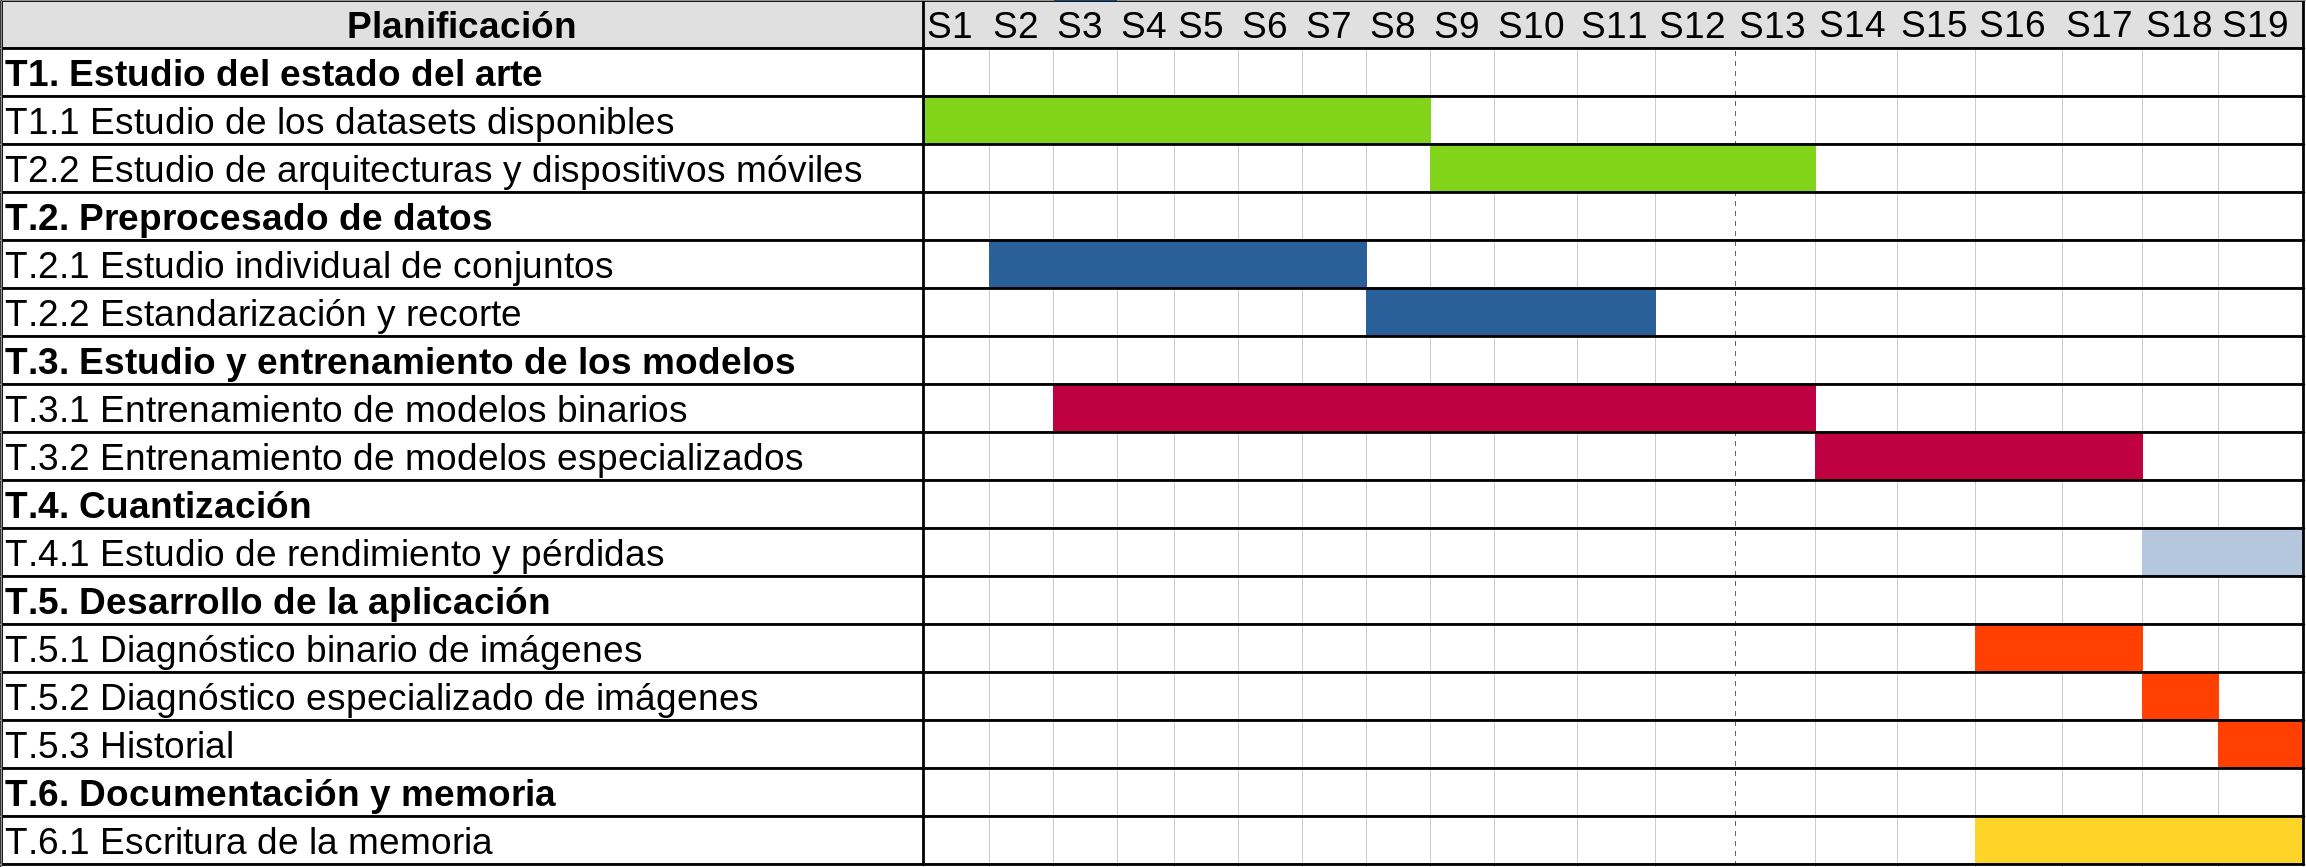
\includegraphics[scale = 0.1755]{imagenes/ganttplan.png}
	\caption{Diagrama de Gantt de planificación}
	\label{fig:gantt}
\end{figure}


Podemos observar también el desglose en subtareas realizado para cada una de las tareas realizadas, que han dado como resultado final la realización y completado del proyecto.

Las reuniones de seguimiento y planificación se han desarrollado en un período medio de 2 semanas entre reuniones, de forma que existiese tiempo suficiente para realizar avances medibles. En dichas reuniones, se trataban los avances realizados, y los problemas encontrados, de forma que se pudiera poner remedio a ellos durante el siguiente \textit{sprint}.